% Options for packages loaded elsewhere
\PassOptionsToPackage{unicode}{hyperref}
\PassOptionsToPackage{hyphens}{url}
\PassOptionsToPackage{dvipsnames,svgnames,x11names}{xcolor}
%
\documentclass[
  xelatex,
  ja=standard]{bxjsarticle}

\usepackage{amsmath,amssymb}
\usepackage{iftex}
\ifPDFTeX
  \usepackage[T1]{fontenc}
  \usepackage[utf8]{inputenc}
  \usepackage{textcomp} % provide euro and other symbols
\else % if luatex or xetex
  \usepackage{unicode-math}
  \defaultfontfeatures{Scale=MatchLowercase}
  \defaultfontfeatures[\rmfamily]{Ligatures=TeX,Scale=1}
\fi
\usepackage{lmodern}
\ifPDFTeX\else  
    % xetex/luatex font selection
  \setmainfont[BoldFont=Noto Sans CJK JP]{Noto Serif CJK JP}
\fi
% Use upquote if available, for straight quotes in verbatim environments
\IfFileExists{upquote.sty}{\usepackage{upquote}}{}
\IfFileExists{microtype.sty}{% use microtype if available
  \usepackage[]{microtype}
  \UseMicrotypeSet[protrusion]{basicmath} % disable protrusion for tt fonts
}{}
\makeatletter
\@ifundefined{KOMAClassName}{% if non-KOMA class
  \IfFileExists{parskip.sty}{%
    \usepackage{parskip}
  }{% else
    \setlength{\parindent}{0pt}
    \setlength{\parskip}{6pt plus 2pt minus 1pt}}
}{% if KOMA class
  \KOMAoptions{parskip=half}}
\makeatother
\usepackage{xcolor}
\setlength{\emergencystretch}{3em} % prevent overfull lines
\setcounter{secnumdepth}{5}
% Make \paragraph and \subparagraph free-standing
\ifx\paragraph\undefined\else
  \let\oldparagraph\paragraph
  \renewcommand{\paragraph}[1]{\oldparagraph{#1}\mbox{}}
\fi
\ifx\subparagraph\undefined\else
  \let\oldsubparagraph\subparagraph
  \renewcommand{\subparagraph}[1]{\oldsubparagraph{#1}\mbox{}}
\fi


\providecommand{\tightlist}{%
  \setlength{\itemsep}{0pt}\setlength{\parskip}{0pt}}\usepackage{longtable,booktabs,array}
\usepackage{calc} % for calculating minipage widths
% Correct order of tables after \paragraph or \subparagraph
\usepackage{etoolbox}
\makeatletter
\patchcmd\longtable{\par}{\if@noskipsec\mbox{}\fi\par}{}{}
\makeatother
% Allow footnotes in longtable head/foot
\IfFileExists{footnotehyper.sty}{\usepackage{footnotehyper}}{\usepackage{footnote}}
\makesavenoteenv{longtable}
\usepackage{graphicx}
\makeatletter
\def\maxwidth{\ifdim\Gin@nat@width>\linewidth\linewidth\else\Gin@nat@width\fi}
\def\maxheight{\ifdim\Gin@nat@height>\textheight\textheight\else\Gin@nat@height\fi}
\makeatother
% Scale images if necessary, so that they will not overflow the page
% margins by default, and it is still possible to overwrite the defaults
% using explicit options in \includegraphics[width, height, ...]{}
\setkeys{Gin}{width=\maxwidth,height=\maxheight,keepaspectratio}
% Set default figure placement to htbp
\makeatletter
\def\fps@figure{htbp}
\makeatother

\renewcommand{\thefootnote}{\arabic{footnote}}
\makeatletter
\@ifpackageloaded{tcolorbox}{}{\usepackage[skins,breakable]{tcolorbox}}
\@ifpackageloaded{fontawesome5}{}{\usepackage{fontawesome5}}
\definecolor{quarto-callout-color}{HTML}{909090}
\definecolor{quarto-callout-note-color}{HTML}{0758E5}
\definecolor{quarto-callout-important-color}{HTML}{CC1914}
\definecolor{quarto-callout-warning-color}{HTML}{EB9113}
\definecolor{quarto-callout-tip-color}{HTML}{00A047}
\definecolor{quarto-callout-caution-color}{HTML}{FC5300}
\definecolor{quarto-callout-color-frame}{HTML}{acacac}
\definecolor{quarto-callout-note-color-frame}{HTML}{4582ec}
\definecolor{quarto-callout-important-color-frame}{HTML}{d9534f}
\definecolor{quarto-callout-warning-color-frame}{HTML}{f0ad4e}
\definecolor{quarto-callout-tip-color-frame}{HTML}{02b875}
\definecolor{quarto-callout-caution-color-frame}{HTML}{fd7e14}
\makeatother
\makeatletter
\makeatother
\makeatletter
\makeatother
\makeatletter
\@ifpackageloaded{caption}{}{\usepackage{caption}}
\AtBeginDocument{%
\ifdefined\contentsname
  \renewcommand*\contentsname{目次}
\else
  \newcommand\contentsname{目次}
\fi
\ifdefined\listfigurename
  \renewcommand*\listfigurename{図一覧}
\else
  \newcommand\listfigurename{図一覧}
\fi
\ifdefined\listtablename
  \renewcommand*\listtablename{表一覧}
\else
  \newcommand\listtablename{表一覧}
\fi
\ifdefined\figurename
  \renewcommand*\figurename{図}
\else
  \newcommand\figurename{図}
\fi
\ifdefined\tablename
  \renewcommand*\tablename{表}
\else
  \newcommand\tablename{表}
\fi
}
\@ifpackageloaded{float}{}{\usepackage{float}}
\floatstyle{ruled}
\@ifundefined{c@chapter}{\newfloat{codelisting}{h}{lop}}{\newfloat{codelisting}{h}{lop}[chapter]}
\floatname{codelisting}{コード}
\newcommand*\listoflistings{\listof{codelisting}{コード一覧}}
\makeatother
\makeatletter
\@ifpackageloaded{caption}{}{\usepackage{caption}}
\@ifpackageloaded{subcaption}{}{\usepackage{subcaption}}
\makeatother
\makeatletter
\@ifpackageloaded{tcolorbox}{}{\usepackage[skins,breakable]{tcolorbox}}
\makeatother
\makeatletter
\@ifundefined{shadecolor}{\definecolor{shadecolor}{rgb}{.97, .97, .97}}
\makeatother
\makeatletter
\makeatother
\makeatletter
\makeatother
\ifLuaTeX
\usepackage[bidi=basic]{babel}
\else
\usepackage[bidi=default]{babel}
\fi
\babelprovide[main,import]{japanese}
% get rid of language-specific shorthands (see #6817):
\let\LanguageShortHands\languageshorthands
\def\languageshorthands#1{}
\ifLuaTeX
  \usepackage{selnolig}  % disable illegal ligatures
\fi
\usepackage[]{natbib}
\bibliographystyle{jecon}
\IfFileExists{bookmark.sty}{\usepackage{bookmark}}{\usepackage{hyperref}}
\IfFileExists{xurl.sty}{\usepackage{xurl}}{} % add URL line breaks if available
\urlstyle{same} % disable monospaced font for URLs
\hypersetup{
  pdftitle={人権保障},
  pdfauthor={土井翔平},
  pdflang={ja},
  colorlinks=true,
  linkcolor={NavyBlue},
  filecolor={Maroon},
  citecolor={NavyBlue},
  urlcolor={NavyBlue},
  pdfcreator={LaTeX via pandoc}}

\title{人権保障}
\usepackage{etoolbox}
\makeatletter
\providecommand{\subtitle}[1]{% add subtitle to \maketitle
  \apptocmd{\@title}{\par {\large #1 \par}}{}{}
}
\makeatother
\subtitle{国際公共政策学}
\author{土井翔平}
\date{2023-07-19}

\begin{document}
\maketitle
\ifdefined\Shaded\renewenvironment{Shaded}{\begin{tcolorbox}[boxrule=0pt, interior hidden, breakable, enhanced, borderline west={3pt}{0pt}{shadecolor}, sharp corners, frame hidden]}{\end{tcolorbox}}\fi

\hypertarget{ux306fux3058ux3081ux306b}{%
\section*{はじめに}\label{ux306fux3058ux3081ux306b}}
\addcontentsline{toc}{section}{はじめに}

17-18世紀の啓蒙思想家\(\leadsto\)人が生まれながらにして持っている\textbf{自然権}
(natural rights)

\begin{tcolorbox}[enhanced jigsaw, bottomtitle=1mm, toptitle=1mm, toprule=.15mm, arc=.35mm, coltitle=black, bottomrule=.15mm, colframe=quarto-callout-note-color-frame, opacitybacktitle=0.6, colbacktitle=quarto-callout-note-color!10!white, breakable, leftrule=.75mm, left=2mm, title=\textcolor{quarto-callout-note-color}{\faInfo}\hspace{0.5em}{アメリカ独立宣言(1776年)}, rightrule=.15mm, titlerule=0mm, opacityback=0, colback=white]

われわれは、以下の事実を自明のことと信じる。すなわち、すべての人間は\textbf{生まれながらにして平等}であり、その創造主によって、生命、自由、および幸福の追求を含む\textbf{不可侵の権利}を与えられているということ。

\end{tcolorbox}

\begin{tcolorbox}[enhanced jigsaw, bottomtitle=1mm, toptitle=1mm, toprule=.15mm, arc=.35mm, coltitle=black, bottomrule=.15mm, colframe=quarto-callout-note-color-frame, opacitybacktitle=0.6, colbacktitle=quarto-callout-note-color!10!white, breakable, leftrule=.75mm, left=2mm, title=\textcolor{quarto-callout-note-color}{\faInfo}\hspace{0.5em}{フランス人権宣言(1789年)}, rightrule=.15mm, titlerule=0mm, opacityback=0, colback=white]

フランス人権宣言 人は、\textbf{自由かつ諸権利において平等なもの}として生まれ、そして生存する。

\end{tcolorbox}

\begin{itemize}
\tightlist
\item
  なぜ人権は保障されないのか?
\item
  なぜ他国の人権保障に関心を持つのか?
\item
  どのように国際的な人権保障に取り組んでいるのか?
\end{itemize}

\hypertarget{ux4ebaux6a29ux306eux56fdux969bux5316}{%
\section{人権の国際化}\label{ux4ebaux6a29ux306eux56fdux969bux5316}}

\hypertarget{ux7b2cux4e8cux6b21ux4e16ux754cux5927ux6226ux307eux3067}{%
\subsection{第二次世界大戦まで}\label{ux7b2cux4e8cux6b21ux4e16ux754cux5927ux6226ux307eux3067}}

人権問題=国内問題/主権国家体系の下で他国の国内問題に干渉することは\textbf{内政不干渉原則}?

\begin{itemize}
\tightlist
\item
  国家主権の契機となったウェストファリア条約

  \begin{itemize}
  \tightlist
  \item
    宗教戦争であった30年戦争
  \item
    領主の信仰の自由
  \end{itemize}
\item
  内政問題を口実とした戦争を回避するためのメカニズムとしての主権
\end{itemize}

\(\leadsto\)国家主権の下で人権侵害/国際社会からの批判をかわす口実

内政問題である人権問題に対して国際社会が無関心ではいられない?

\begin{itemize}
\tightlist
\item
  19世紀における奴隷制度の廃止運動
\item
  第1次世界大戦後の民族自決と少数民族
\item
  産業化における労働者の保護
\end{itemize}

\begin{figure}[htpb]

{\centering \includegraphics{human_rights_files/mediabag/800px-Map_Europe_192.png}

}

\caption{\href{https://commons.wikimedia.org/wiki/File:Map_Europe_1923-en.svg}{1923年のヨーロッパ}}

\end{figure}

\hypertarget{ux7b2cux4e8cux6b21ux4e16ux754cux5927ux6226ux5f8c}{%
\subsection{第二次世界大戦後}\label{ux7b2cux4e8cux6b21ux4e16ux754cux5927ux6226ux5f8c}}

ナチス・ドイツによるユダヤ人虐殺(\textbf{ホロコースト})\(\leadsto\)人権が国際問題として認知

\begin{itemize}
\tightlist
\item
  第2次世界大戦は自由主義とファシズムの戦い(ということになっていた)。
\end{itemize}

\(\leadsto\)国連憲章においても人権に関する言及、国際関心事項

\begin{tcolorbox}[enhanced jigsaw, bottomtitle=1mm, toptitle=1mm, toprule=.15mm, arc=.35mm, coltitle=black, bottomrule=.15mm, colframe=quarto-callout-note-color-frame, opacitybacktitle=0.6, colbacktitle=quarto-callout-note-color!10!white, breakable, leftrule=.75mm, left=2mm, title=\textcolor{quarto-callout-note-color}{\faInfo}\hspace{0.5em}{\href{https://www.unic.or.jp/info/un/charter/text_japanese/}{国連憲章} 第55条}, rightrule=.15mm, titlerule=0mm, opacityback=0, colback=white]

人民の同権及び自決の原則の尊重に基礎をおく諸国間の平和的且つ友好的関係に必要な安定及び福祉の条件を創造するために、国際連合は、次のことを促進しなければならない。

\begin{enumerate}
\def\labelenumi{\alph{enumi}.}
\setcounter{enumi}{2}
\tightlist
\item
  人種、性、言語又は宗教による差別のないすべての者のための\textbf{人権及び基本的自由の普遍的な尊重及び遵守}
\end{enumerate}

\end{tcolorbox}

\begin{itemize}
\tightlist
\item
  国連総会第3委員会
\end{itemize}

1948年に国連総会が\href{https://www.unic.or.jp/activities/humanrights/document/bill_of_rights/universal_declaration/}{\textbf{世界人権宣言}}
(Universal Declaration of Human Rights; A/RES/217 (III)) を採択

\begin{itemize}
\tightlist
\item
  第1,2条は人間の尊厳に関する基本原則
\item
  第3-19条は市民的自由
\item
  第20-27条は政治的・社会的・経済的平等
\item
  第28,29条は集団としての権利
\end{itemize}

国連総会決議\(\leadsto\)法的拘束力はない/現在の国際人権法の基盤

最初の国際人権条約は\href{https://worldjpn.grips.ac.jp/documents/texts/mt/19481209.T1J.html}{\textbf{ジェノサイド条約}}(1948年採択、1951年発効)

\begin{itemize}
\tightlist
\item
  \textbf{集団殺害} (genocide) が定義
\item
  国際法上の犯罪であるとしてその防止と処罰が義務付け
\item
  日本は批准せず
\end{itemize}

\begin{figure}[htpb]

{\centering \includegraphics{figures/convention_genocide.jpg}

}

\caption{\href{https://www.un.org/en/genocideprevention/genocide-convention.shtml}{ジェノサイド条約締約国}}

\end{figure}

\hypertarget{ux56fdux969bux4ebaux6a29ux7ae0ux5178}{%
\subsection{国際人権章典}\label{ux56fdux969bux4ebaux6a29ux7ae0ux5178}}

世界人権宣言\(\leadsto\)
2つの人権規約が1966年に採択、1976年に発効\footnote{日本では社会権規約をA規約、自由権規約をB規約と呼ぶことがある。}

\begin{itemize}
\tightlist
\item
  \href{https://www.nichibenren.or.jp/activity/international/library/human_rights/liberty_convention.html}{\textbf{自由権規約}}
  (International Covenant on Civil and Political Rights)
\item
  \href{https://www.nichibenren.or.jp/activity/international/library/human_rights/society_convention.html}{\textbf{社会権規約}}
  (International Covenant on Economic, Social and Cultural Rights)
\end{itemize}

\(\leadsto\)\href{https://www.unic.or.jp/activities/humanrights/document/bill_of_rights/}{\textbf{国際人権章典}}
(International Bill of Human
Rights):世界人権宣言と自由権規約、社会権規約および選択議定書

人権=\textbf{自由権}+\textbf{社会権}

\begin{itemize}
\tightlist
\item
  自由権:国家が市民の生活や政治活動に介入しないことで保障される権利
\end{itemize}

\begin{figure}[htpb]

{\centering \includegraphics{human_rights_files/mediabag/800px-ICCPR-members2.PNG}

}

\caption{\href{https://commons.wikimedia.org/wiki/File:ICCPR-members2.PNG}{自由権規約締約国}}

\end{figure}

\begin{itemize}
\tightlist
\item
  社会権:市民の経済的・社会的・文化的活動を支援することで保障される権利
\end{itemize}

\begin{figure}[htpb]

{\centering \includegraphics{human_rights_files/mediabag/800px-ICESCR_members.png}

}

\caption{\href{https://commons.wikimedia.org/wiki/File:ICESCR_members.svg}{社会権規約締約国}}

\end{figure}

その後も\href{https://www.ohchr.org/en/core-international-human-rights-instruments-and-their-monitoring-bodies}{様々な人権条約}および追加議定書
(optional protocol) が締結\(\leadsto\)包括的な国際人権法が形成

\hypertarget{ux81eaux7531ux6a29ux306eux4fddux969c}{%
\subsection{自由権の保障}\label{ux81eaux7531ux6a29ux306eux4fddux969c}}

\begin{figure}[htpb]

{\centering 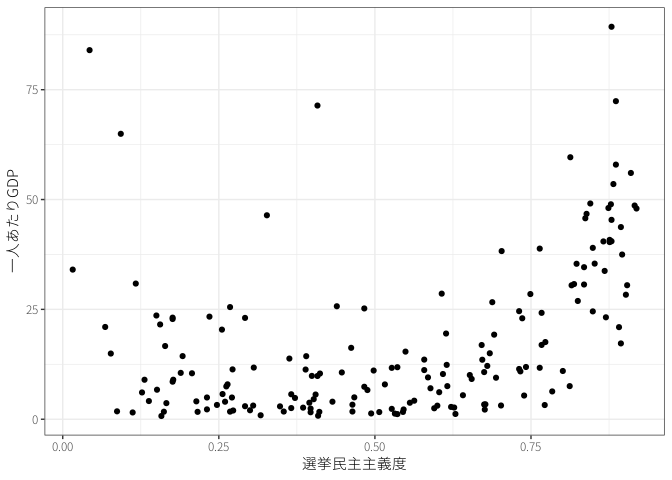
\includegraphics{human_rights_files/figure-pdf/unnamed-chunk-2-1.png}

}

\caption{自由権保障の推移}

\end{figure}

\begin{figure}[htpb]

{\centering 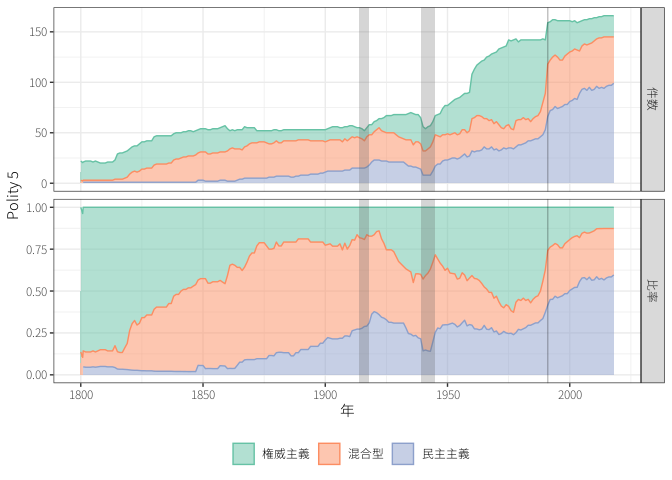
\includegraphics{human_rights_files/figure-pdf/unnamed-chunk-3-1.png}

}

\caption{自由権保障の水準}

\end{figure}

\hypertarget{ux4ebaux6a29ux4fddux969cux3092ux5de1ux308bux653fux6cbb}{%
\section{人権保障を巡る政治}\label{ux4ebaux6a29ux4fddux969cux3092ux5de1ux308bux653fux6cbb}}

人権は生まれながらにして全ての人間が持っている権利\(\leadsto\)\textbf{普遍的}
(universal)

ただし、\textbf{どのような権利を、どの程度保障すべきなのか}についての考えは時代や地域によって異なる。

\begin{itemize}
\tightlist
\item
  冷戦期:西側諸国は政治的自由に関する自由権/東側諸国は平等や社会保障に関する社会権を重視
\item
  人権を重視する国でも(アメリカのように)テロリストへの拷問
\item
  自由権は平等で自律的な個人を前提とした西洋的価値観に基づいている?
\item
  \(\leadsto\)他の地域では十分には受け入れがたい?

  \begin{itemize}
  \tightlist
  \item
    東アジア諸国が成長\(\leadsto\)「\textbf{アジア的価値観} (Asian
    value) 」

    \begin{itemize}
    \tightlist
    \item
      アジアでは個人の自由よりも家族や社会の発展、調和を優先
    \item
      既存の国際人権法は西洋的価値観の押し付け、内政干渉
    \end{itemize}
  \item
    自由主義諸国はこうした考えは権威主義体制を正当化するに過ぎないと批判
  \end{itemize}
\item
  自由権を第1世代の人権、社会権を第2世代の人権とも呼ぶ
\item
  第3世代の人権:\href{https://www.unic.or.jp/activities/humanrights/promotion_protection/development/}{発展の権利}、平和への権利など集団として人権
\end{itemize}

人権は普遍的/国際人権法も普遍的あるいは中立的なものではない\(\leadsto\)国際的な人権保障を巡る政治が存在

\hypertarget{ux56fdux5bb6ux306bux3088ux308bux4ebaux6a29ux4fb5ux5bb3}{%
\subsection{国家による人権侵害}\label{ux56fdux5bb6ux306bux3088ux308bux4ebaux6a29ux4fb5ux5bb3}}

ベルギーのレオポルド2世:19世紀末から20世紀初頭にかけてのコンゴ自由国の苛烈な統治

\begin{itemize}
\tightlist
\item
  象牙や天然ゴムの生産のために先住民を強制的に労働・厳しい処罰
\item
  レオポルド2世が邪悪な性格であったり、ベルギー本国でも独裁的であったわけではない。
\end{itemize}

ミャンマーの民主派のアウンサンスーチーがリーダーになってもロヒンギャへの弾圧は継続

\begin{figure}

\begin{minipage}[t]{0.50\linewidth}

{\centering 

\raisebox{-\height}{

\includegraphics{human_rights_files/mediabag/400px-Leopold_ii_gar.jpg}

}

\caption{レオポルド2世}

}

\end{minipage}%
%
\begin{minipage}[t]{0.50\linewidth}

{\centering 

\raisebox{-\height}{

\includegraphics{human_rights_files/mediabag/400px-Remise_du_Prix.jpg}

}

\caption{アウンサン・スー・チー}

}

\end{minipage}%

\end{figure}

\(\leadsto\)人権侵害が起こる理由は政治家の性格だけでなく、国内政治にもある?

\begin{enumerate}
\def\labelenumi{\arabic{enumi}.}
\tightlist
\item
  財政が乏しく社会保障を整備できない/軍隊や警察へのコントロールが不十分\citep{cole2015}
\item
  国家安全保障を理由(あるいは口実)とした人権の制約\citep{poe1994, krain1997}

  \begin{itemize}
  \tightlist
  \item
    政府に対する抗議を犯罪として取り締まり/適切な手続き (due process)
    なしの裁判
  \item
    敵対国の出身者(WW2における在米日系人)やテロリスト容疑者(ドローンによる標的殺害)を不当に拘束、殺害
  \item
    テロリズム予防のために市民のプライバシーを侵害(愛国者法)
  \end{itemize}
\item
  権威主義国や新興民主主義国\citep{davenport1995}において政権の維持のために反政府勢力や他民族を弾圧

  \begin{itemize}
  \tightlist
  \item
    民主主義国:選挙を通じて平和的に政権交代ができる\(\leadsto\)反政府活動は起こりにくい
  \item
    一党独裁や個人独裁の国:反政府活動を抑止できる\(\leadsto\)人権侵害が起こりにくい
  \item
    多党独裁の国:政治的競争がある\(\leadsto\)人権侵害\citep{vreeland2008}
  \end{itemize}
\end{enumerate}

\hypertarget{ux4ebaux6a29ux6761ux7d04ux3078ux306eux53c2ux52a0}{%
\subsection{人権条約への参加}\label{ux4ebaux6a29ux6761ux7d04ux3078ux306eux53c2ux52a0}}

\begin{figure}[htpb]

{\centering 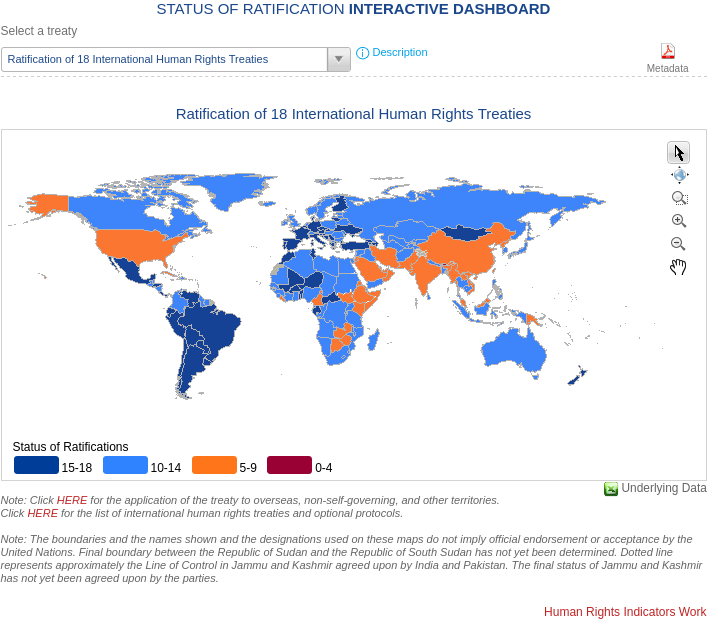
\includegraphics[width=0.8\textwidth,height=\textheight]{figures/human_rights_treaty.png}

}

\caption{\href{https://indicators.ohchr.org}{主要人権条約の締結数}}

\end{figure}

\begin{itemize}
\tightlist
\item
  新興民主主義国:人権条約に批准\(\leadsto\)人権侵害のコストを高める\(\leadsto\)政治体制を維持\citep{moravcsik2000}
\item
  成熟した民主主義国:既に人権保障を行っている\(\leadsto\)わざわざ人権条約を批准しない
\item
  権威主義国:条約に違反しても制裁はない\(\leadsto\)評判のために批准
\end{itemize}

民主主義国は民主化や人権保障を条件に他国に利益を供与

\begin{itemize}
\tightlist
\item
  北大西洋条約機構や欧州連合では民主主義や人権保障、自由経済などを加盟要件
\item
  トルコやハンガリーのようにEUへの加盟を目指して、あるいは追放を恐れて人権保障に取り組むとは限らない。
\end{itemize}

\hypertarget{ux4ed6ux56fdux306eux4ebaux6a29ux554fux984c}{%
\subsection{他国の人権問題}\label{ux4ed6ux56fdux306eux4ebaux6a29ux554fux984c}}

なぜ\textbf{他国の人権環境が改善しても直接の利益にはならないにもかかわらず}、他国の人権保障に関心を持つのか?

\begin{enumerate}
\def\labelenumi{\arabic{enumi}.}
\tightlist
\item
  道徳的理由

  \begin{itemize}
  \tightlist
  \item
    人々は弱者に対して共感、同情する社会的生き物
  \item
    他国の人権侵害を看過\(\leadsto\)人権が侵害されてもよい状況や人々があることを認める\(\leadsto\)自身への人権侵害を許容
  \item
    人権は普遍的なものであるという規範の内面化
  \item
    情報通信技術の発達、特にSNS\(\leadsto\)人々は他国の人権問題に関心を持たざるを得ない
  \end{itemize}
\item
  戦略的理由

  \begin{itemize}
  \tightlist
  \item
    他国が人権を保障\(\leadsto\)(さらには民主化することにより)国際的な平和と経済繁栄が実現\(\leadsto\)自国の国益
  \item
    周辺国の人権侵害\(\leadsto\)内戦など\(\leadsto\)近隣諸国に戦火の拡大や難民の流出で被害
  \item
    地域貿易協定に労働者の権利に関する条項\(\leadsto\)途上国の労働環境を改善\(\leadsto\)先進国の労働者の競争力を向上\citep{hafner2005a}
  \end{itemize}
\end{enumerate}

\hypertarget{ux4ebaux6a29ux306eux56fdux969bux5316ux306eux80ccux666f}{%
\subsection{人権の国際化の背景}\label{ux4ebaux6a29ux306eux56fdux969bux5316ux306eux80ccux666f}}

なぜ\textbf{内政不干渉原則に抵触するにもかかわらず}、国家は人権の国際化を(部分的に)受け入れたのか?

\(\leadsto\)道徳的理由と戦略的理由から絡み合って「意図せず」人権の地位向上\citep[第2章]{tsutsui2022}

\begin{itemize}
\tightlist
\item
  第2次世界大戦後の植民地独立(民族自決)と差別撤廃
\item
  人権条約の軽視ゆえの批准\(\leadsto\)国際人権としての地位\citep{hafner2005b}
\item
  体制間競争における非難の口実

  \begin{itemize}
  \tightlist
  \item
    アメリカにおける人種問題、ソ連(東側)における政治的不自由
  \end{itemize}
\item
  国際人権NGOの活動\citep{tsutsui2004}
\end{itemize}

\textbf{越境的アドボカシー・ネットワーク} (transnational advocacy
network) や\textbf{規範起業家} (norm
entrepreneur):特定の規範を普及させようとする人々や集団

\begin{itemize}
\tightlist
\item
  \href{https://www.mofa.go.jp/mofaj/gaiko/arms/mine/genjo.html}{対人地雷禁止条約}、\href{https://www.mofa.go.jp/mofaj/gaiko/treaty/shomei_37.html}{クラスター弾禁止条約}
\end{itemize}

\textbf{規範ライフ・サイクル}:国際規範は3段階に従って発展する\citep{finnemore1998}

\begin{enumerate}
\def\labelenumi{\arabic{enumi}.}
\tightlist
\item
  規範起業家は自らの信念を他者と共有するために活動
\item
  信念を共有する人々の数が転換点 (tipping point)
  \(\leadsto\)\textbf{規範カスケード}:多くの人々が規範として受け入れ、それに反する行為は批判
\item
  規範が内面化 (internalized)
  され、当然のものに(それに従うという意識すらなくなる)
\end{enumerate}

\begin{figure}

\begin{minipage}[t]{0.50\linewidth}

{\centering 

\raisebox{-\height}{

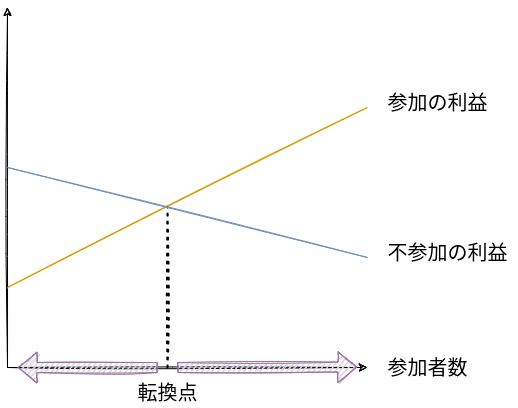
\includegraphics{figures/tipping_point1.drawio.png}

}

\caption{規範カスケードのイメージ}

}

\end{minipage}%
%
\begin{minipage}[t]{0.50\linewidth}

{\centering 

\raisebox{-\height}{

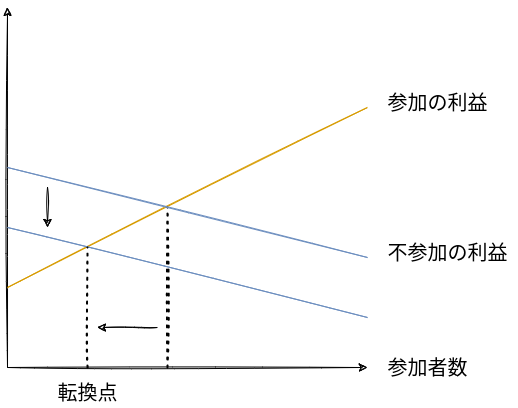
\includegraphics{figures/tipping_point2.drawio.png}

}

\caption{規範カスケードのイメージ}

}

\end{minipage}%

\end{figure}

\begin{itemize}
\tightlist
\item
  グローバル・スタンダードも同じメカニズム
\end{itemize}

\hypertarget{ux56fdux969bux7684ux306aux4ebaux6a29ux4fddux969c}{%
\section{国際的な人権保障}\label{ux56fdux969bux7684ux306aux4ebaux6a29ux4fddux969c}}

一般的に国際制度に意味があるのかは見解が分かれている。

\begin{itemize}
\tightlist
\item
  アナーキーな国際社会では国家に制度の遵守を強制することはできない\(\leadsto\)制度には国家の行動に影響する効果はない\citep{mearsheimer2017}
\item
  ほとんどの国はほとんどの時期においてほとんどのルールに従っている\citep{henkin1979}

  \begin{itemize}
  \tightlist
  \item
    国際制度に意味がないのであれば、わざわざ国家が時間や労力をかけて交渉する意味は>
  \item
    制度に違反するのは遵守する能力が欠如していたり、制度が曖昧である\(\leadsto\)不遵守\citep{chayes1993}
  \item
    国際制度は国家が同意したものである\(\leadsto\)遵守できるルールが制度として形になっているだけ\citep{downs1996}
  \end{itemize}
\end{itemize}

\hypertarget{ux4ebaux6a29ux6761ux7d04ux306eux52b9ux679c}{%
\subsection{人権条約の効果}\label{ux4ebaux6a29ux6761ux7d04ux306eux52b9ux679c}}

人権条約の効果を検証する上での問題1:人権侵害の発見

\begin{itemize}
\tightlist
\item
  一般的に、人権侵害は外部から確認しにくい
\item
  \href{https://www.amnesty.or.jp/}{Amnesty
  International}や\href{https://jp.usembassy.gov/ja/category/reports-ja/}{アメリカ国務省}のレポートに依拠\footnote{\href{http://www.humanrightsdata.com/}{CIRI
    Human Rights Data Project}}
\end{itemize}

これらの情報が網羅的かつ正しいとししても、人権侵害の基準が時代と共に変化するかも?

\begin{itemize}
\tightlist
\item
  人権規範が浸透する\(\leadsto\)人権侵害とみなされていなかった行為がそうであるとみなされる
\item
  技術革新・リソースの向上\(\leadsto\)多くの人権侵害の「発見」
\item
  時間変化を考慮して分析すると、(拷問の禁止に関する)人権保障の程度は改善\citep{fariss2014}
\end{itemize}

\begin{figure}[htpb]

{\centering 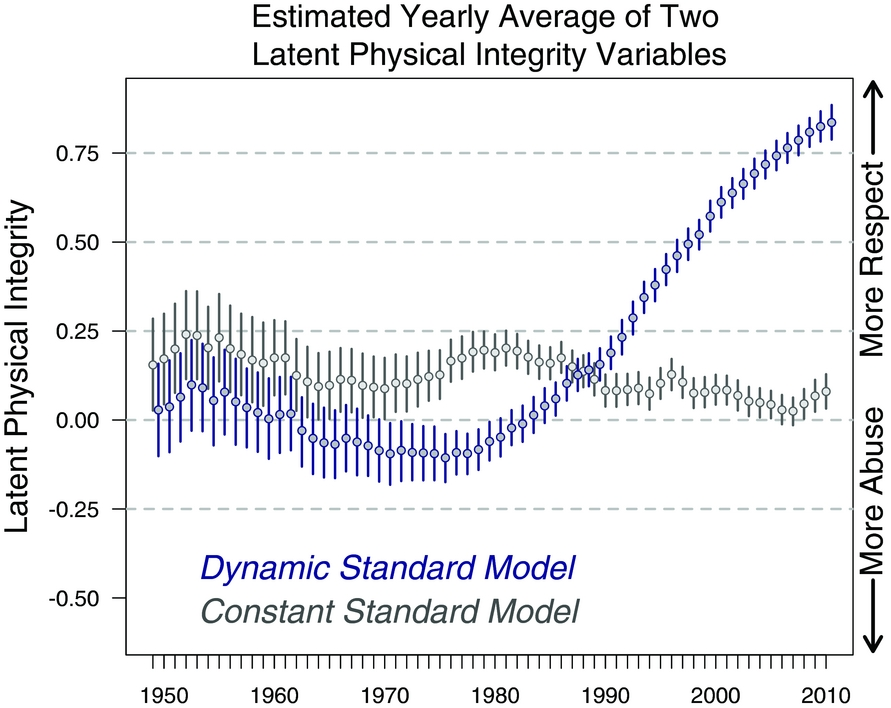
\includegraphics{figures/fariss.jpeg}

}

\caption{\citet{fariss2014}}

\end{figure}

人権条約の効果を検証する上での問題2:自己選択

\begin{itemize}
\tightlist
\item
  人権保障に熱心な国家が人権条約に批准?\(\leadsto\)見かけの相関
\item
  例:民主主義国や経済的に豊かな国
\end{itemize}

第3の要因を考慮して分析すると人権条約は効果がないか、負の効果があるという研究\citep{keith1999, hathaway2001, hafner2005b, hill2010}

\begin{itemize}
\tightlist
\item
  人権条約に強制力はなし/人権を保障させるために圧力を欠ける国は少ない
\item
  人権条約への批准は人権を保障するという評判を得るため
\item
  多党独裁の国:反体制派の影響力が高い\(\leadsto\)人権条約に批准する/弾圧のために人権を侵害
\end{itemize}

一方で、人権条約の効果は特定の条件において生じるという見方\citep{neumayer2005, murdie2012, conrad2013, lupu2013}

人権条約の短期的効果は小さいが、長期的な効果があるという見解\citep{hafner2007, tsutsui2012}

\begin{itemize}
\tightlist
\item
  人権問題を国際問題として扱う土壌

  \begin{itemize}
  \tightlist
  \item
    人権条約がなければ人権NGOは人権侵害の評価もできない。
  \item
    国家は\textbf{評判} (reputation)
    を気にする\(\leadsto\)NGOをはじめとする越境的アドボカシー・ネットワークによる\textbf{名指しと非難}
    (naming and shaming) に効果がある?\citep{hafner2008}

    \begin{itemize}
    \tightlist
    \item
      \href{https://freedomhouse.org/}{Freedom
      House}や\href{https://www.hrw.org/ja}{Human Rights
      Watch}も代表的な人権NGO
    \item
      \textbf{ブーメラン・モデル}:外国の政府やNGO、国際機構を通じて自国の政府に圧力をかける\citep{keck1999}
    \end{itemize}
  \item
    1975年の\href{https://www.mofa.go.jp/mofaj/area/osce/gaiyo.html}{欧州安全保障協力会議}
    (Conference on Security and Cooperation in Europe:
    CSCE)のヘルシンキ宣言:東西で領土保全、経済交流、人権保障に合意\(\leadsto\)共産主義国内における人権活動の活発化
  \end{itemize}
\end{itemize}

\begin{figure}[htpb]

{\centering 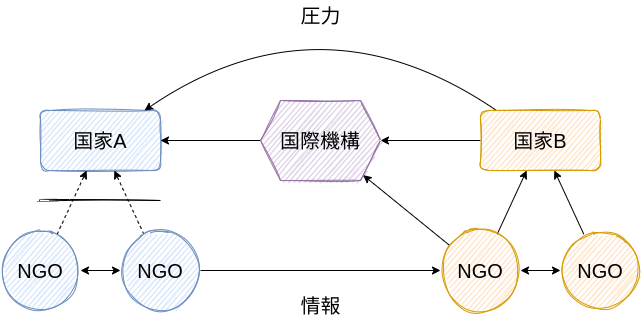
\includegraphics{figures/boomerang_model.drawio.png}

}

\caption{ブーメラン・モデルのイメージ}

\end{figure}

\hypertarget{ux4ebaux6a29ux5236ux88c1}{%
\subsection{人権制裁}\label{ux4ebaux6a29ux5236ux88c1}}

外部からの圧力、制裁\(\leadsto\)人権条約を遵守

\begin{itemize}
\tightlist
\item
  経済制裁をする国が被る費用<他国の人権状況の改善という利益?
\end{itemize}

いくつかの条件の下で、国家は人権制裁を行うと考えられる。

\begin{enumerate}
\def\labelenumi{\arabic{enumi}.}
\tightlist
\item
  国内から他国の人権状況の改善のために行動するよう政治的圧力

  \begin{itemize}
  \tightlist
  \item
    越境的アボドカシー・ネットワークは市民に外国の人権問題を注意喚起
  \end{itemize}
\item
  敵対国で人権侵害
\item
  内政不干渉原則を越えるような価値と結合

  \begin{itemize}
  \tightlist
  \item
    民族浄化や人種差別は人権問題を越えて民族自決権や反植民地主義といった価値の問題?
  \end{itemize}
\end{enumerate}

共同で人権制裁=囚人のジレンマ

\begin{itemize}
\tightlist
\item
  協力して制裁をすれば改善する/他国の制裁にタダ乗り
\end{itemize}

南アフリカの\href{https://www.unic.or.jp/activities/humanrights/discrimination/apartheid/}{\textbf{アパルトヘイト撤廃}}は経済制裁による人権問題の解決の数少ない例

\begin{figure}

\begin{minipage}[t]{0.50\linewidth}

{\centering 

\raisebox{-\height}{

\includegraphics{human_rights_files/mediabag/49_apartheid.jpg}

}

\caption{\href{https://www.mofa.go.jp/mofaj/press/pr/wakaru/topics/vol49/index.html}{アパルトヘイト関連法}}

}

\end{minipage}%
%
\begin{minipage}[t]{0.50\linewidth}

{\centering 

\raisebox{-\height}{

\includegraphics{human_rights_files/mediabag/49_nenpyou.jpg}

}

\caption{\href{https://www.mofa.go.jp/mofaj/press/pr/wakaru/topics/vol49/index.html}{アパルトヘイト撤廃の流れ}}

}

\end{minipage}%

\end{figure}

制裁\(\leadsto\)無辜の市民に被害?

\begin{itemize}
\tightlist
\item
  政治的エリートのみを標的とする\textbf{スマート制裁}
\item
  十分な効果を上げられるのか、本当にエリートのみに制裁を加えられるのか?
\end{itemize}

\hypertarget{ux56fdux969bux7684ux5be9ux67fb}{%
\subsection{国際的審査}\label{ux56fdux969bux7684ux5be9ux67fb}}

\hypertarget{ux4ebaux6a29ux7406ux4e8bux4f1a}{%
\subsubsection{人権理事会}\label{ux4ebaux6a29ux7406ux4e8bux4f1a}}

国際連合の\href{https://www.mofa.go.jp/mofaj/gaiko/jinken_r/index.html}{\textbf{人権理事会}}
(Human Rights Council) や国連人権高等弁務官事務所 (Office of the High
Commissioner for Human Rights: OHCHR)
:加盟国の人権状況を包括的に監視、審査

\begin{figure}[htpb]

{\centering 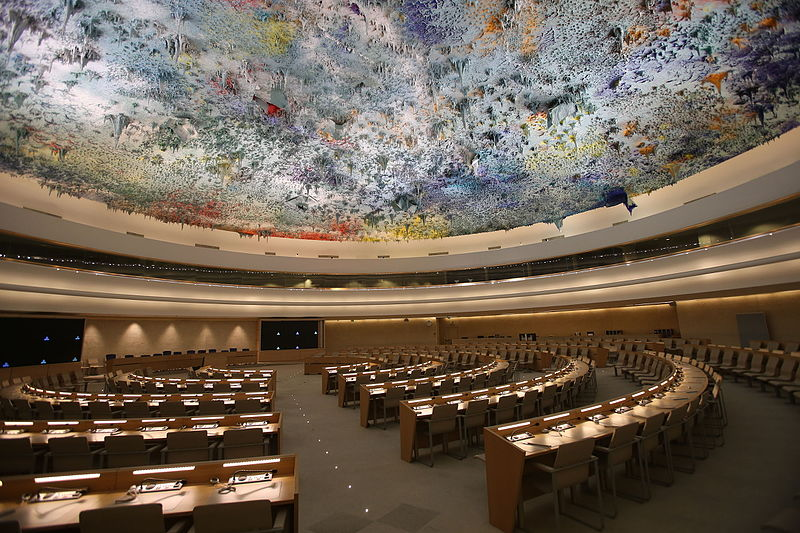
\includegraphics{figures/human_rights_council.jpg}

}

\caption{\href{https://commons.wikimedia.org/wiki/File:UN_Geneva_Human_Rights_and_Alliance_of_Civilizations_Room.jpg}{国連人権理事会}}

\end{figure}

\begin{itemize}
\tightlist
\item
  人権理事会は2006年に国連人権委員会から改組
\item
  \href{https://www.mofa.go.jp/mofaj/gaiko/jinken_r/upr_gai.html}{\textbf{普遍的定期審査}}
  (Universal Periodic Review: UPR):加盟国の人権状況を審査する中心的活動
\item
  他にも国別あるいはテーマ別の特別手続きや個人による不服申立手続きなど
\item
  専門家からなる人権理事会諮問委員会から助言
\end{itemize}

人権侵害を行っているとされている国も理事国になるなどの問題も

\hypertarget{ux4ebaux6a29ux6761ux7d04ux306eux59d4ux54e1ux4f1a}{%
\subsubsection{人権条約の委員会}\label{ux4ebaux6a29ux6761ux7d04ux306eux59d4ux54e1ux4f1a}}

人権条約ごとにも委員会が設置され、締約国の履行を確認

\begin{itemize}
\tightlist
\item
  自由権規約や社会権規約では、専門家からなる自由権(社会権)規約委員会に国家が履行状況を定期的に報告し、委員会が審査
\end{itemize}

最も洗礼された人権の国際的な保障手続きとして\textbf{個人請願}
(individual petition)

\begin{itemize}
\tightlist
\item
  1950年に欧州評議会加盟国が欧州人権条約に批准

  \begin{itemize}
  \tightlist
  \item
    人権侵害を受けている加盟国の市民が欧州人権裁判所で訴訟
  \end{itemize}
\item
  自由権規約第1選択議定書や社会権規約選択議定書の締約国国民は\textbf{個人通報制度}
  (individual complaints mechanism) を利用可
\end{itemize}

\hypertarget{ux4f01ux696dux306bux3088ux308bux4ebaux6a29ux4fddux969c}{%
\subsubsection{企業による人権保障}\label{ux4f01ux696dux306bux3088ux308bux4ebaux6a29ux4fddux969c}}

多くの場合、人権侵害を行うのは国家であるが、近年は企業による人権侵害にも関心

\begin{itemize}
\tightlist
\item
  2011年に人権理事会は\href{https://www.mofa.go.jp/mofaj/gaiko/bhr/index.html}{ビジネスと人権に関する指導原則}を採択\(\leadsto\)企業にも人権尊重を求める

  \begin{itemize}
  \tightlist
  \item
    一部の国ではこれに従って\href{https://www.ohchr.org/en/special-procedures/wg-business/national-action-plans-business-and-human-rights}{行動計画}を策定
  \end{itemize}
\item
  \href{https://www.unglobalcompact.org/}{国連グローバル・コンパクト}:人権、労働、環境、腐敗防止に関する10の原則を掲げ、企業は自発的に参加し、進捗の報告
\item
  \href{https://www.unpri.org/}{国連責任投資原則}:6つのESG投資に関する原則を掲げ、投資家に遵守を呼びかけ
\item
  \href{https://www.globalreporting.org/}{グローバル・レポーティング・イニシアティブ}:経済、環境、社会に与える影響の報告基準を策定
\end{itemize}

\(\leadsto\)政治的パワーがなくても国際規範を作り、企業に遵守させることは可能?

\hypertarget{ux65e5ux672cux306eux4ebaux6a29ux72b6ux6cc1}{%
\section[日本の人権状況]{\texorpdfstring{日本の人権状況\footnote{具体的な日本の人権問題については
  \citet{shin2020} を参照。}}{日本の人権状況}}\label{ux65e5ux672cux306eux4ebaux6a29ux72b6ux6cc1}}

\href{https://elaws.e-gov.go.jp/document?lawid=321CONSTITUTION}{日本国憲法}:第11条に基本的人権の保障が明記、第3章に具体的な権利が列挙

\begin{itemize}
\tightlist
\item
  国際的に見ると、制定当初は人権規定が豊富/一度も改正されず、現在ではやや少ない\footnote{ケネス・盛・マッケルウェイン\href{https://www.nippon.com/ja/in-depth/a05602/}{「日本国憲法:その特異な歩みと構造」}}
\end{itemize}

\begin{figure}[htpb]

{\centering \includegraphics{human_rights_files/mediabag/26941.png}

}

\caption{日本国憲法の特徴}

\end{figure}

日本は\href{https://www.hurights.or.jp/archives/treaty/un-treaty-list.html}{全ての人権条約に批准しているわけではない}

\begin{itemize}
\tightlist
\item
  例:ジェノサイド条約/個人通報制度を定める自由権規約および社会権規約の\href{https://www.nichibenren.or.jp/activity/international/library/human_rights/liberty_protocols_no1.html}{第一選択議定書}/死刑撤廃を定める自由権規約第二選択議定書など
\end{itemize}

\href{https://www.mofa.go.jp/mofaj/gaiko/bhr/index.html}{ビジネスと人権に関する行動計画}は策定

\href{https://freedomhouse.org/country/japan/freedom-world/2023}{Freedom
House}によると日本は自由が保障(96/100点、2023年現在)

\begin{itemize}
\tightlist
\item
  UPRにおける\href{https://www.nichibenren.or.jp/activity/international/library/upr.html}{報告書}や\href{https://www.mofa.go.jp/mofaj/gaiko/jinken_r/upr_gai.html}{審査結果}や
\item
  個別条約における\href{https://www.nichibenren.or.jp/activity/international/library/human_rights.html}{報告書審査}などで日本の人権問題が指摘
\end{itemize}

\href{https://www.hrw.org/ja/asia/japan}{Human Rights
Watch}などの人権NGOは独自にも人権問題を指摘

\begin{itemize}
\tightlist
\item
  国境なき記者団の\href{https://rsf.org/en/ranking}{報道の自由ランキング}
\end{itemize}

\begin{figure}[htpb]

{\centering 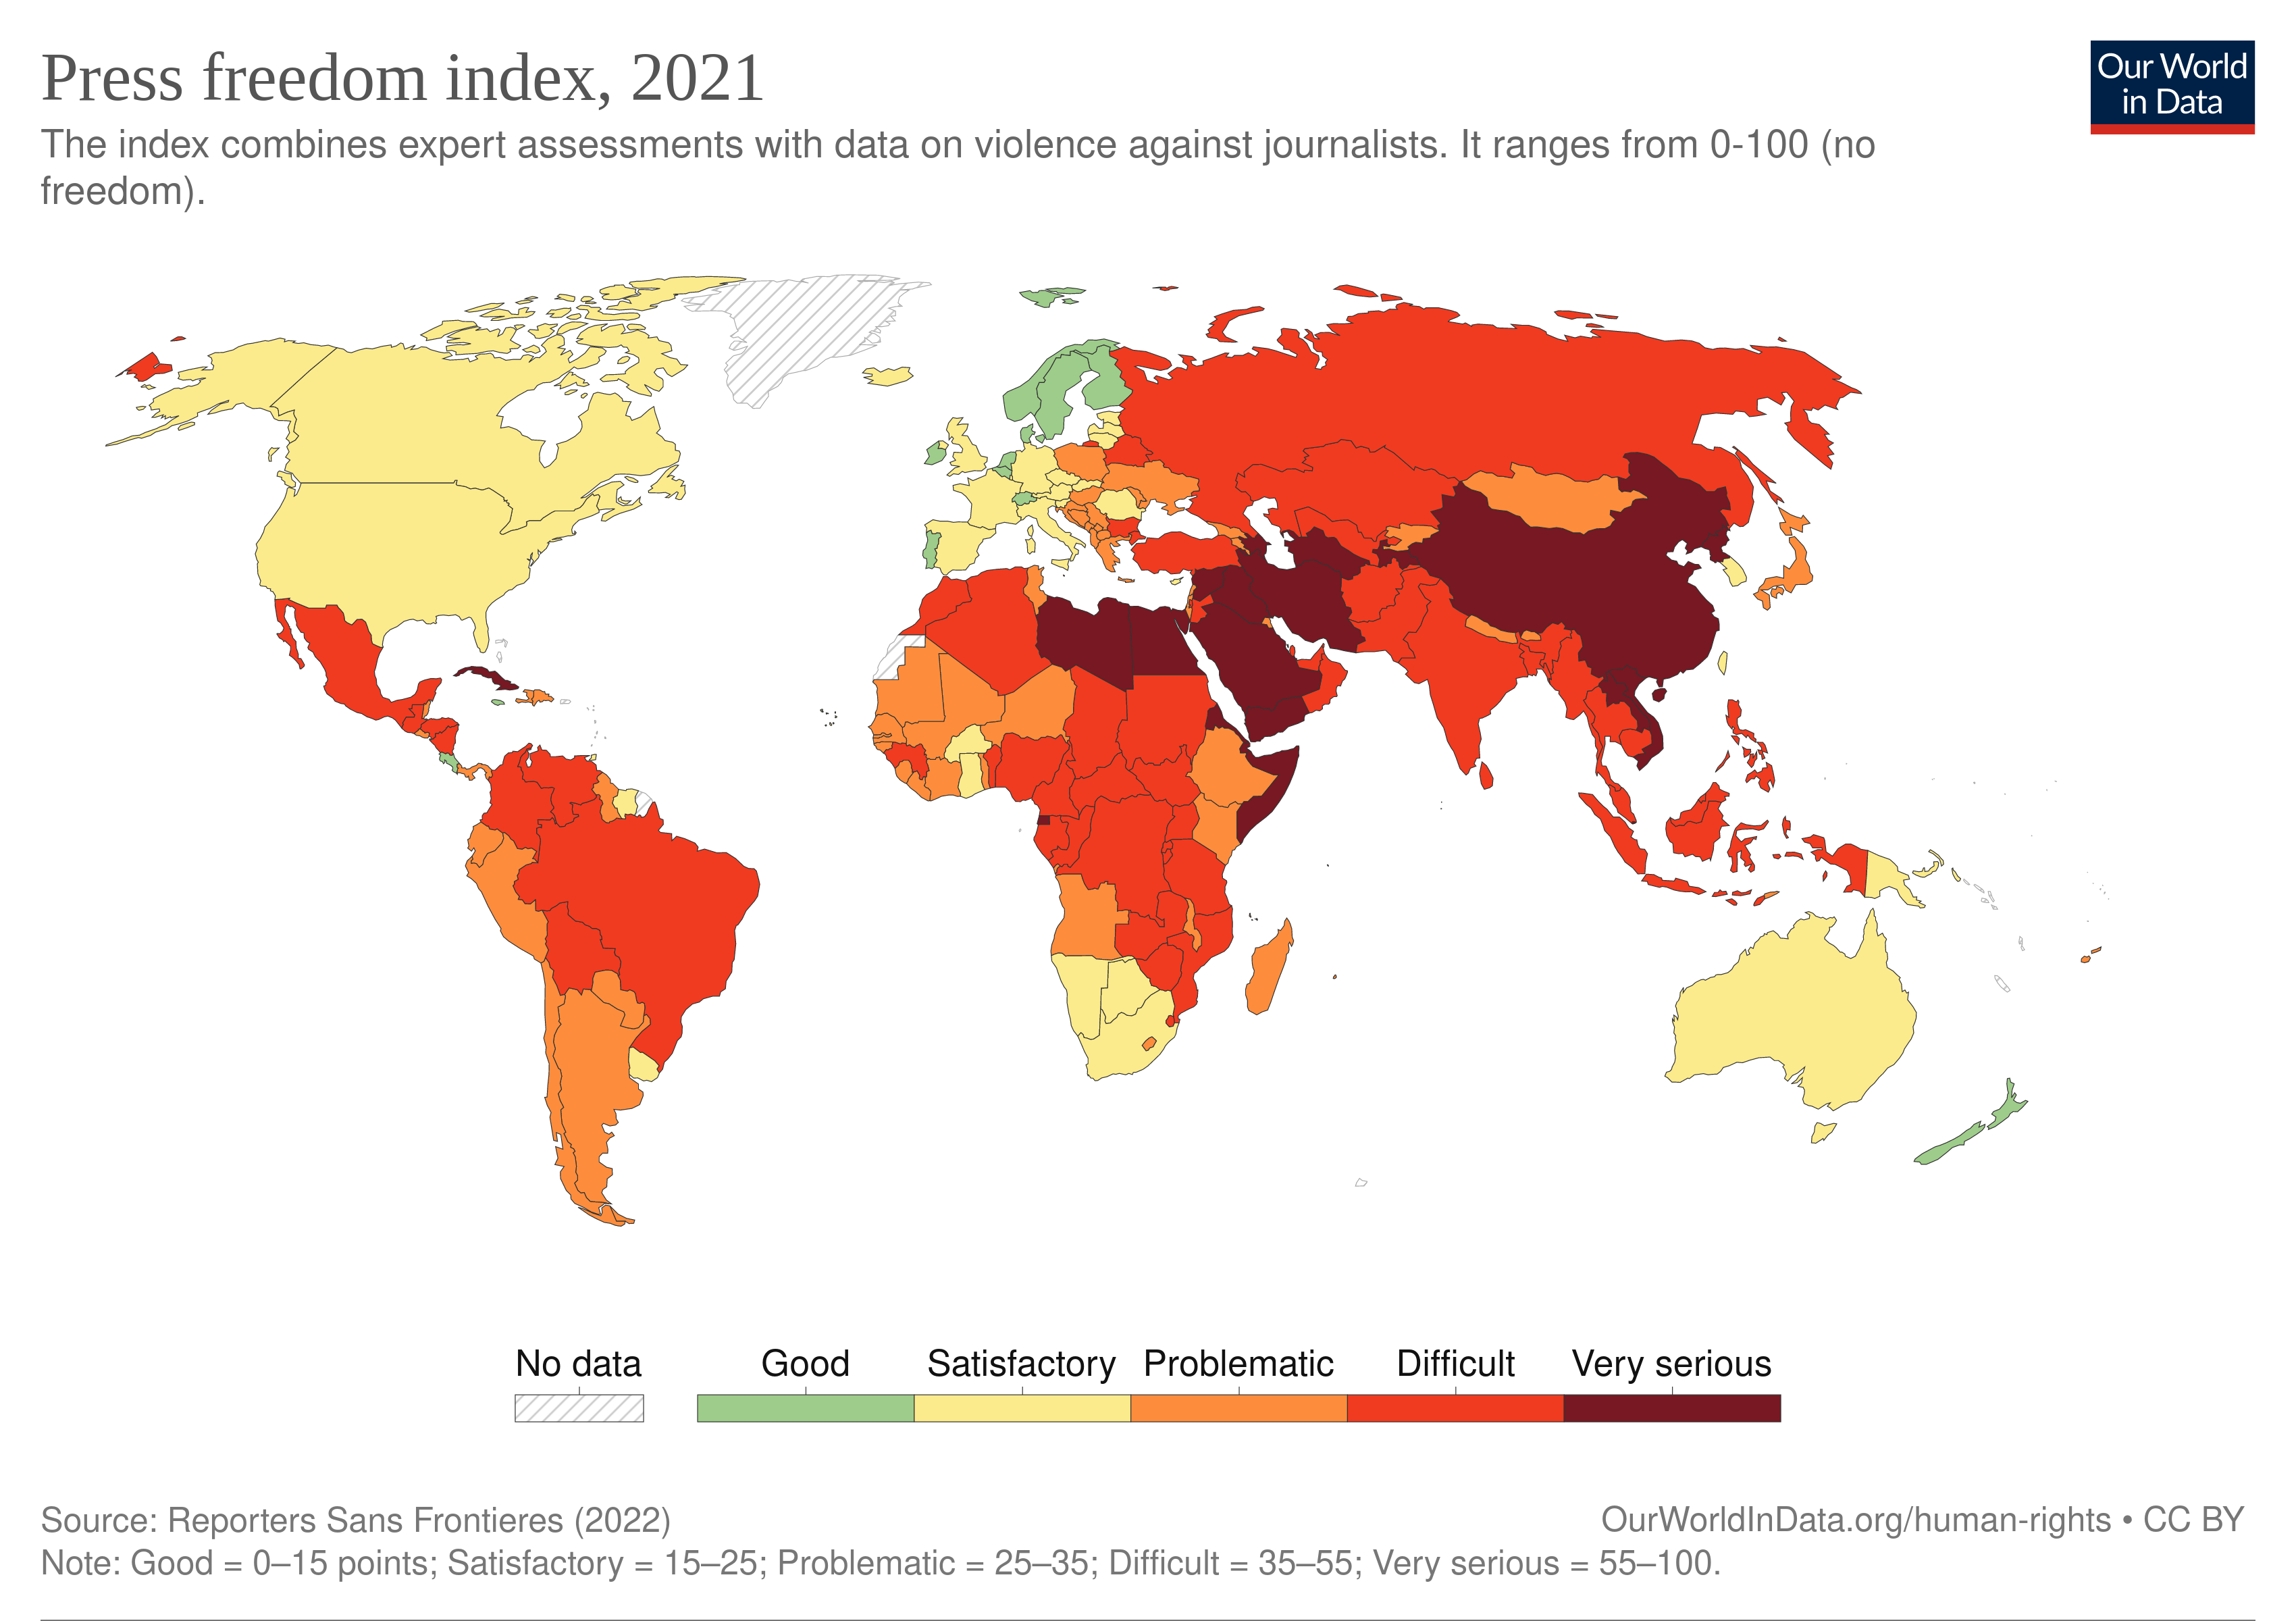
\includegraphics[width=0.8\textwidth,height=\textheight]{figures/press-freedom-index-rsf.png}

}

\caption{報道の自由度(2021年)}

\end{figure}

\begin{itemize}
\tightlist
\item
  世界経済フォーラムの\href{https://jp.weforum.org/reports/global-gender-gap-report-2023}{ジェンダーギャップ指数}
\end{itemize}

\begin{figure}[htpb]

{\centering 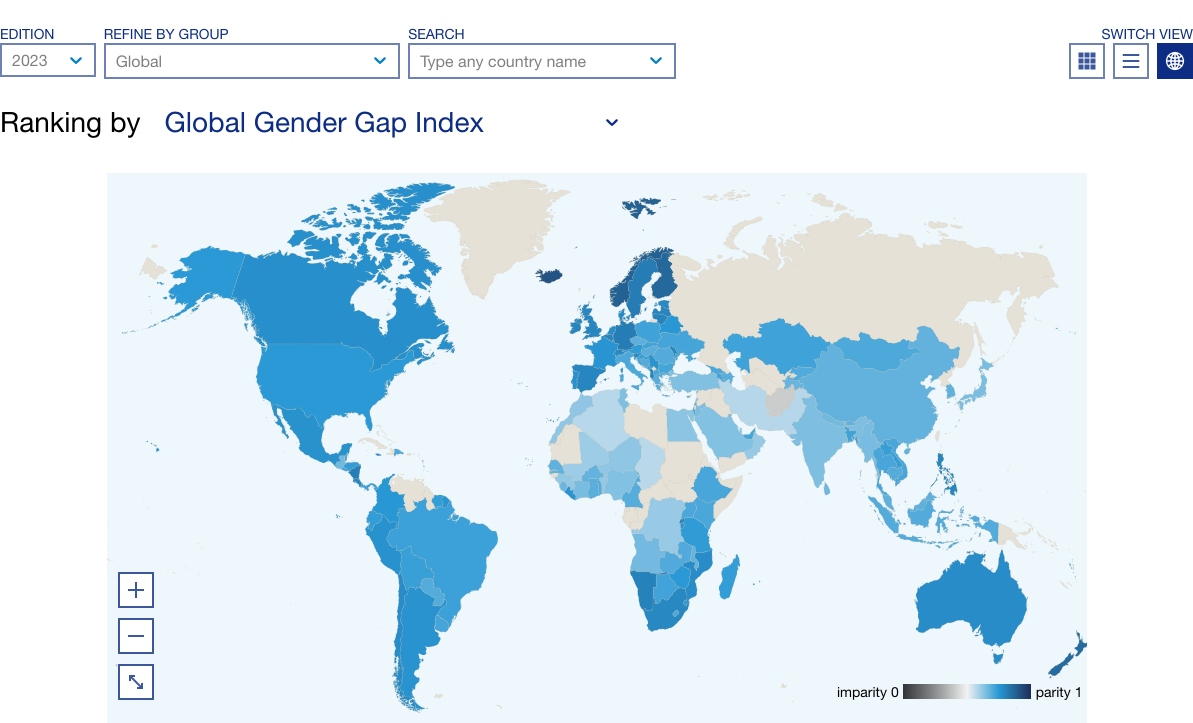
\includegraphics{figures/gender_gap_index.png}

}

\caption{ジェンダーギャップ指数(2023年)}

\end{figure}

\begin{itemize}
\tightlist
\item
  UNDPの\href{https://hdr.undp.org/data-center/thematic-composite-indices/gender-inequality-index\#/indicies/GII}{ジェンダー不平等指数}
\end{itemize}

\begin{figure}[htpb]

{\centering 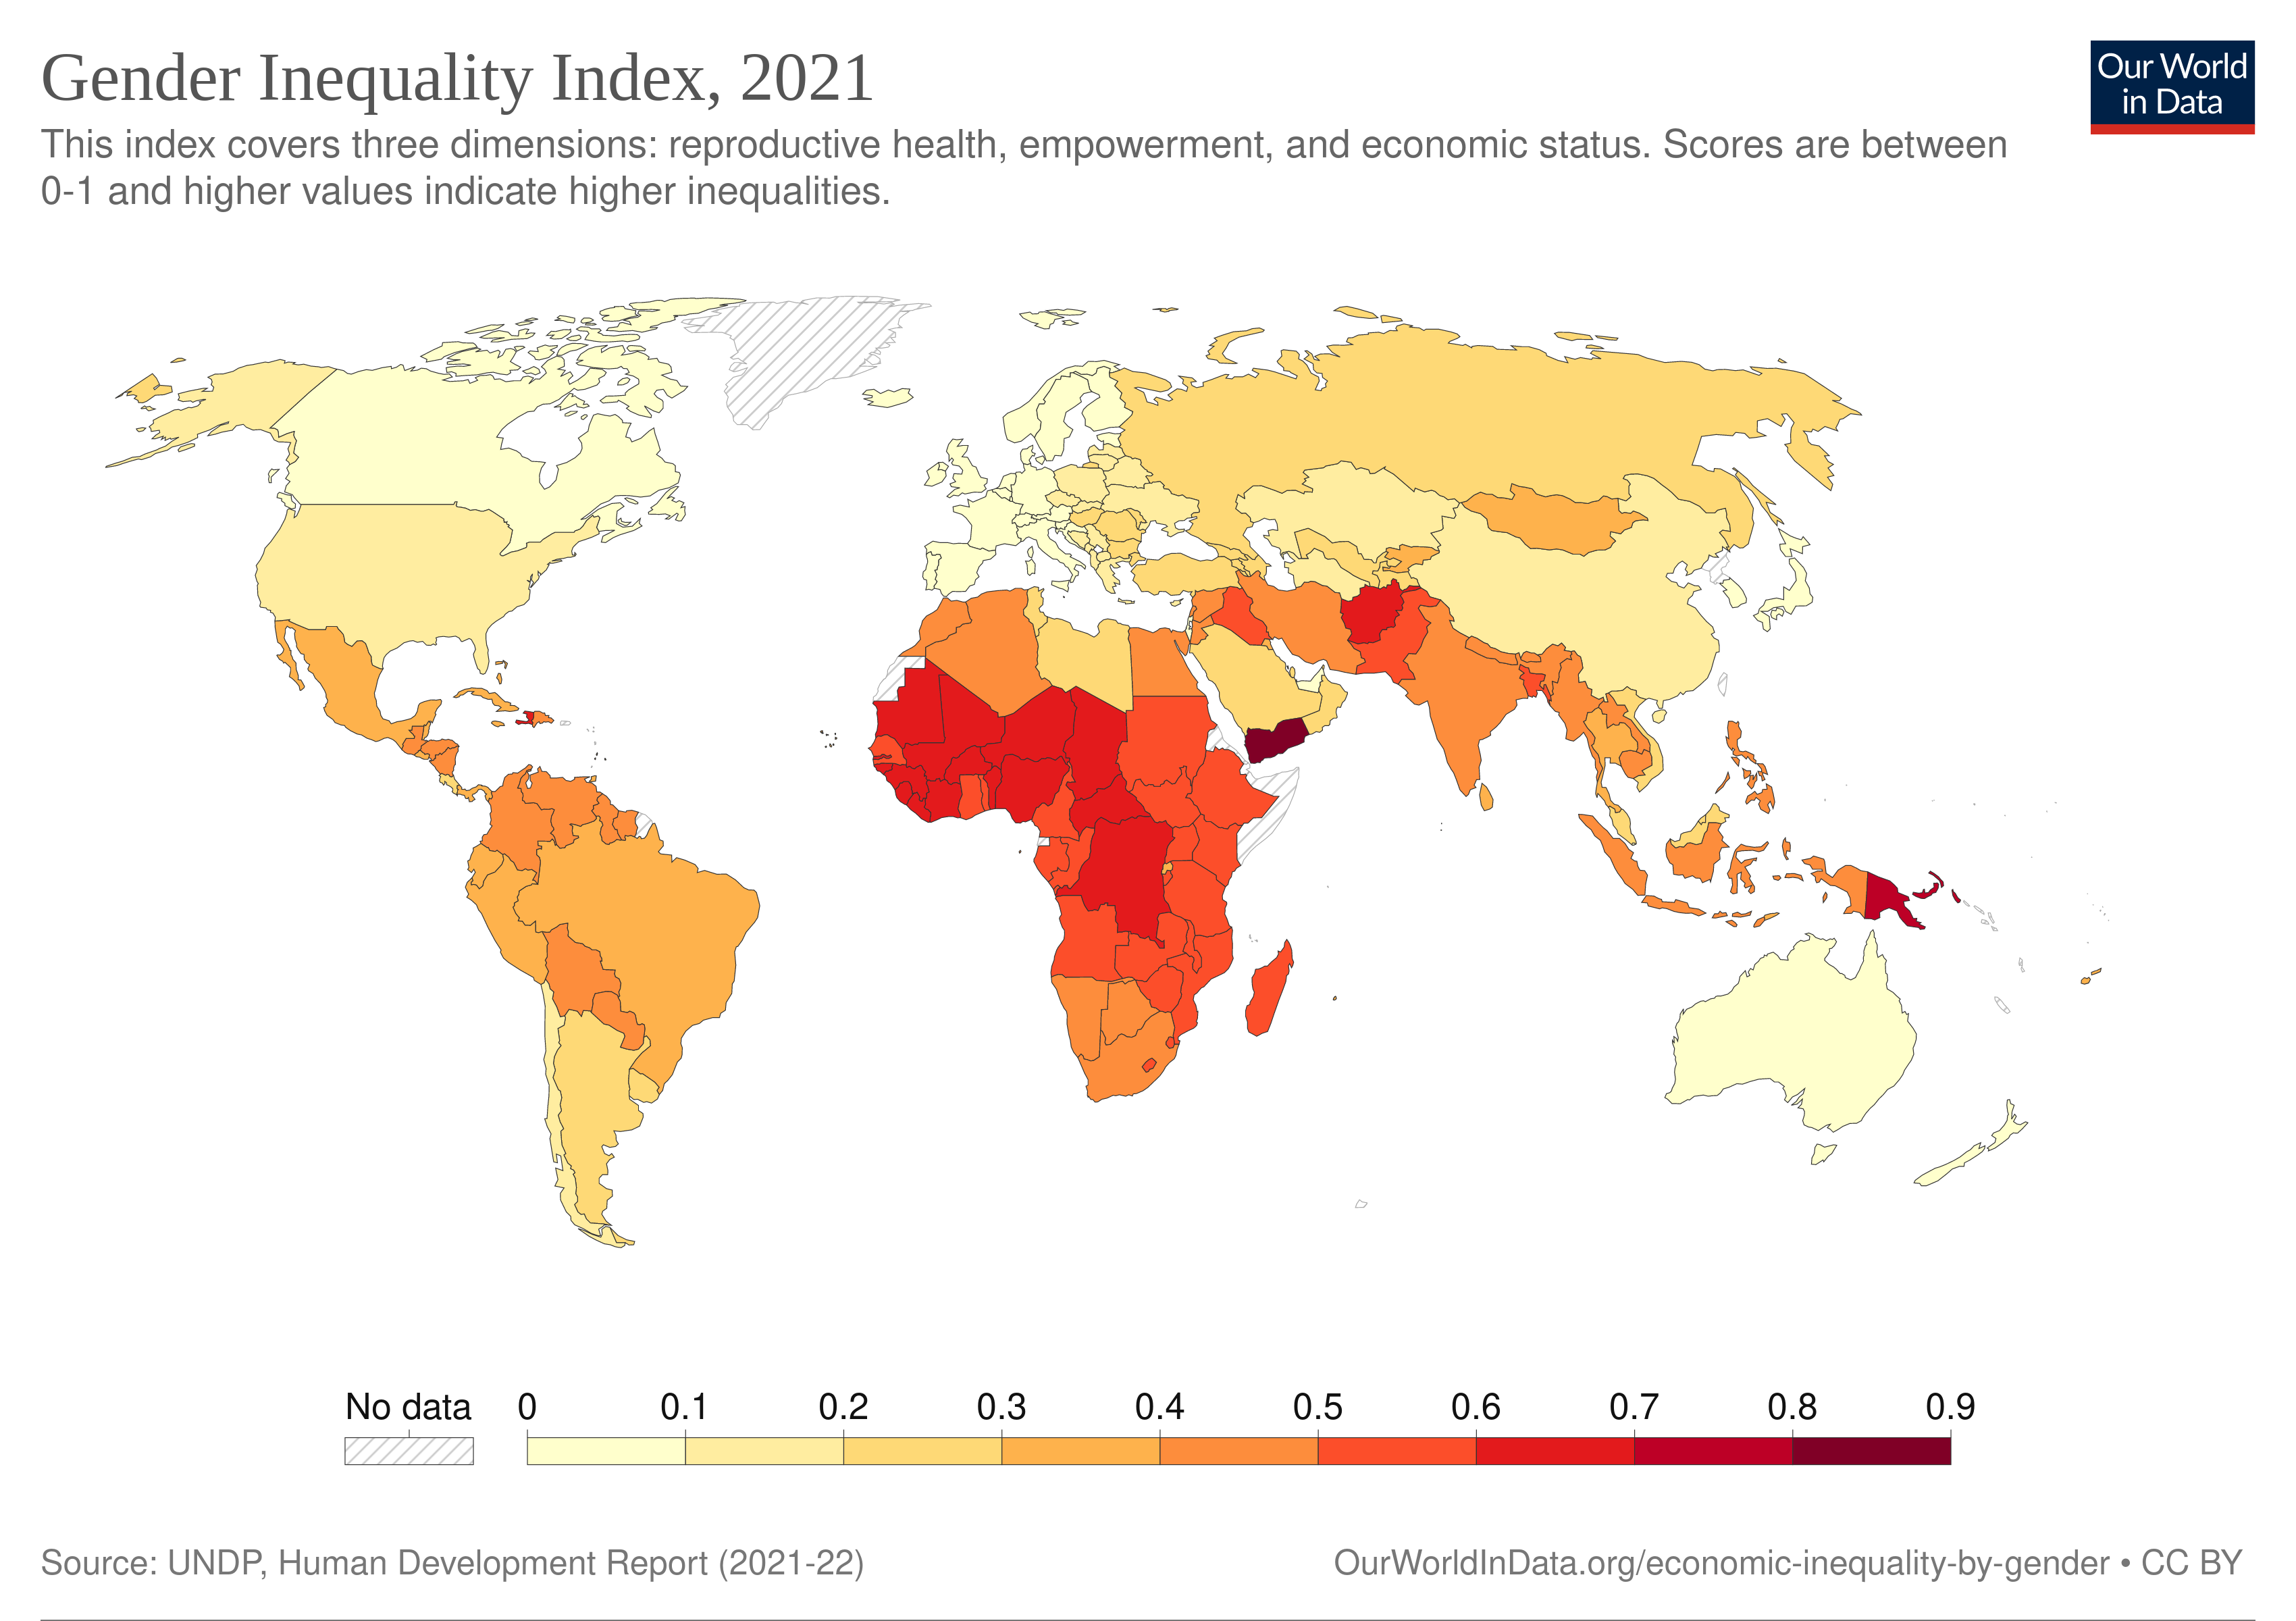
\includegraphics{figures/gender-inequality-index-from-the-human-development-report.png}

}

\caption{ジェンダー不平等指数(2021年)}

\end{figure}

\begin{itemize}
\tightlist
\item
  OECDの\href{https://www.genderindex.org/}{Social Institutions and
  Gender Index}
\end{itemize}

\textbf{アメリカ国務省} (Department of State)
は各国の人権状況の\href{https://jp.usembassy.gov/ja/category/reports-ja/}{報告書}を作成

\hypertarget{ux6226ux4e89ux3068ux4ebaux6a29}{%
\section{戦争と人権}\label{ux6226ux4e89ux3068ux4ebaux6a29}}

\hypertarget{ux5e73ux548cux7dadux6301ux6d3bux52d5ux306eux62e1ux5927}{%
\subsection{平和維持活動の拡大}\label{ux5e73ux548cux7dadux6301ux6d3bux52d5ux306eux62e1ux5927}}

冷戦期に米ソの拒否権によって国連が機能不全\(\leadsto\)\textbf{平和維持活動}
(peacekeeping operation)

\begin{itemize}
\tightlist
\item
  PKO:終結した紛争の停戦や撤退などを監視して、平和が維持するように務める活動
\end{itemize}

\begin{enumerate}
\def\labelenumi{\arabic{enumi}.}
\tightlist
\item
  PKOの受け入れや要因の提供は自発的に行う。
\item
  当事者に対して中立・不偏であり、内政に干渉しない。\\
\item
  武力行使は自衛のために必要最小限に留める。
\end{enumerate}

\begin{itemize}
\tightlist
\item
  戦争を集結させることを目的に介入を行う(第7章下の)強制措置とは異なる。
\end{itemize}

冷戦終結\(\leadsto\)国連への期待の高まり\(\leadsto\)PKOの数も増加

\begin{itemize}
\tightlist
\item
  1992年の「\href{https://www.unic.or.jp/files/peace.pdf}{\textbf{平和への課題}}」:ブトロス=ガリ事務総長は国連の平和機能として予防外交、平和創造、平和維持、平和構築を示す。
\end{itemize}

\hypertarget{ux5e73ux548cux69cbux7bc9}{%
\subsubsection{平和構築}\label{ux5e73ux548cux69cbux7bc9}}

\href{https://www.mofa.go.jp/mofaj/gaiko/peace_b/index.html}{\textbf{平和構築}}
(peacebuilding) :紛争が再発しないような社会を形成していく活動

\begin{itemize}
\tightlist
\item
  武装解除・動員解除・社会復帰 (Disarmament, Demobilization,
  Reintegration: DDR)
  、難民の帰還、文民警察の改革、選挙の実施・監視、統治機構の支援など
\end{itemize}

軍隊による停戦監視を越えて、警察や文民も含めて包括的に平和活動を行うように(\textbf{第2世代PKO}、\textbf{複合型PKO})

\begin{itemize}
\tightlist
\item
  2000年の「\href{https://www.unic.or.jp/files/a_55_305.pdf}{\textbf{ブラヒミ報告}}」:国連の平和活動の中核として位置づけ
\end{itemize}

国連が暫定的に統治を行うことも

\begin{itemize}
\tightlist
\item
  \href{https://www.unic.or.jp/activities/peace_security/action_for_peace/asia_pacific/cambodia/}{カンボジア}

  \begin{itemize}
  \tightlist
  \item
    日本は\href{http://www.moj.go.jp/housouken/houso_houkoku_cambo.html}{カンボジア民法の起草支援}など協力
  \end{itemize}
\item
  \href{https://www.unic.or.jp/activities/peace_security/independence/declaration/east_timor/}{東ティモール}
\item
  \href{https://www.unic.or.jp/activities/peace_security/action_for_peace/europe/kosovo/}{コソボ}など
\end{itemize}

\hypertarget{ux56fdux969bux9078ux6319ux76e3ux8996}{%
\subsubsection{国際選挙監視}\label{ux56fdux969bux9078ux6319ux76e3ux8996}}

選挙の国際的な監視の受け入れは拡大

\begin{figure}[htpb]

{\centering 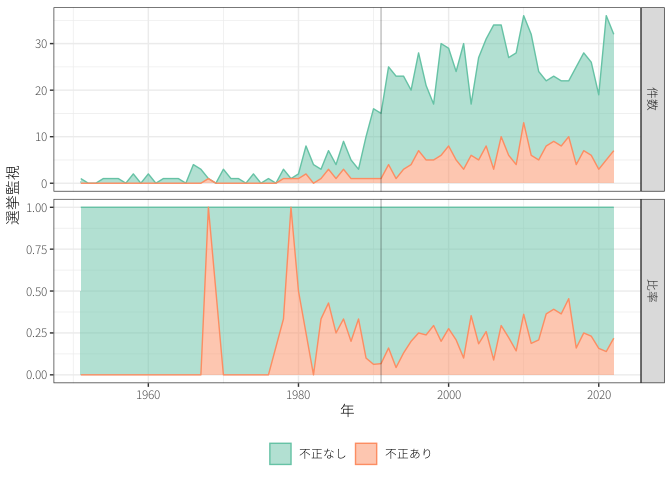
\includegraphics{human_rights_files/figure-pdf/unnamed-chunk-4-1.png}

}

\caption{国際選挙監視と選挙不正}

\end{figure}

\begin{itemize}
\tightlist
\item
  自由で公正な選挙が規範として受け入れられ\(\leadsto\)監視する必要
\item
  名指しと非難\(\leadsto\)選挙監視を受け入れること自体も規範となりつつ\citep{hyde2011}
\end{itemize}

選挙監視によって選挙不正が減少しているかは不明

\begin{itemize}
\tightlist
\item
  選挙権威主義国:監視の受け入れれ(不正が発覚しなければ)\(\leadsto\)民主主義の評判や援助を獲得
\item
  監視されても不正が発覚しない(あるいは発覚しても問題はない)\(\leadsto\)監視を受け入れている可能性。
\end{itemize}

\hypertarget{ux5e73ux548cux5275ux9020ux57f7ux884c}{%
\subsubsection{平和創造(執行)}\label{ux5e73ux548cux5275ux9020ux57f7ux884c}}

平和的手段による解決が不可\(\leadsto\)平和創造 (peace enforcement)
部隊による介入も主張(\textbf{第3世代PKO})

\begin{itemize}
\tightlist
\item
  ユーゴスラビア内戦やソマリア内戦:第7章下の武力行使が認められたPKO
\item
  兵力や装備が不十分、PKO部隊からも死者\(\leadsto\)挫折
\end{itemize}

1995年の「平和への課題:追補」:平和維持や平和構築が強調され、国連独自の平和執行機能は現状では非現実であると認める。

\hypertarget{ux4ebaux9053ux7684ux4ecbux5165}{%
\subsection{人道的介入}\label{ux4ebaux9053ux7684ux4ecbux5165}}

\textbf{人道的介入} (humanitarian
intervention):著しい人権侵害や人道危機を阻止するために当事国の\textbf{同意なく}武力を行使すること

\begin{itemize}
\tightlist
\item
  多くの場合、政府が特定の集団を迫害しているときに介入すべきだと問題に
\end{itemize}

人道危機を放置するわけにはいかない/国家主権を侵害、内政不干渉原則や武力行使禁止原則に違反

\begin{itemize}
\tightlist
\item
  しばしば、自国民や少数民族の保護は武力行使の口実に
\end{itemize}

\hypertarget{ux30e6ux30fcux30b4ux5185ux6226}{%
\subsubsection{ユーゴ内戦}\label{ux30e6ux30fcux30b4ux5185ux6226}}

旧ユーゴスラビア連邦は多民族国家、指導者ティトーの死亡と冷戦終結\(\leadsto\)\textbf{国民国家}
(nation state) に分裂

\begin{figure}[htpb]

{\centering \includegraphics{human_rights_files/mediabag/574px-Yugoslavia_eth.jpg}

}

\caption{\href{https://commons.wikimedia.org/wiki/File:Yugoslavia_ethnic_map.jpg}{1991年のユーゴスラビア連邦における民族分布}}

\end{figure}

\begin{itemize}
\tightlist
\item
  \textbf{民族自決} (self-determination):民族が国家を形成する権利
\end{itemize}

冷戦の終結\(\leadsto\)社会主義国家も民主化を行う/民族対立を助長

\begin{itemize}
\tightlist
\item
  最大民族であるセルビア人に支配されることを他民族は恐れる。
\item
  独立することでセルビア人が他国で少数民族になることをセルビアは恐れる。
\end{itemize}

\(\leadsto\)ユーゴから独立を求める各国とセルビアとの間で内戦

セルビア人によるジェノサイドを\textbf{民族浄化} (ethnic cleansing)
と呼ぶ\(\leadsto\)国際社会からの支持

\begin{itemize}
\tightlist
\item
  セルビア人だけが民族浄化していたわけではない。
\end{itemize}

国連は平和執行部隊を投入するが兵力や情報が足りない\(\leadsto\)人道危機を止めることができず

\begin{itemize}
\tightlist
\item
  特に、スレブレニッツァの悲劇では国連軍の目の前で虐殺\(\leadsto\)国連の限界を知らしめた。
\end{itemize}

スロベニア、クロアチア、ボスニア=ヘルツェゴヴィナは独立する\(\leadsto\)コソボもセルビアからの独立を求めて内戦が再発

\begin{itemize}
\tightlist
\item
  セルビアによるコソボのアルバニア人が虐殺が起こっているとしてNATOが(安保理決議なしに)空爆
\item
  「違法だが正当である」?
\item
  同時期に起こったルワンダ内戦への無関心
\end{itemize}

国家主権/民族自決権/人権のトリレンマ?

\hypertarget{ux4fddux8b77ux3059ux308bux8cacux4efb}{%
\subsubsection{保護する責任}\label{ux4fddux8b77ux3059ux308bux8cacux4efb}}

\href{https://ir.library.osaka-u.ac.jp/repo/ouka/all/67203/}{\textbf{保護する責任}}
(responsibility to protect:
R2P):国家は自国民を保護する責任を持っているが、その責任を果たせ(さ)ない場合、国際社会が代わりに保護

\begin{tcolorbox}[enhanced jigsaw, bottomtitle=1mm, toptitle=1mm, toprule=.15mm, arc=.35mm, coltitle=black, bottomrule=.15mm, colframe=quarto-callout-note-color-frame, opacitybacktitle=0.6, colbacktitle=quarto-callout-note-color!10!white, breakable, leftrule=.75mm, left=2mm, title=\textcolor{quarto-callout-note-color}{\faInfo}\hspace{0.5em}{\href{https://www.mofa.go.jp/mofaj/gaiko/unsokai/pdfs/050916_seika.pdf}{世界サミット成果文書}}, rightrule=.15mm, titlerule=0mm, opacityback=0, colback=white]

\begin{enumerate}
\def\labelenumi{\arabic{enumi}.}
\setcounter{enumi}{137}
\tightlist
\item
  \textbf{各々の国家}は、大量殺戮、戦争犯罪、民族浄化及び人道に対する犯罪からその国の人々を\textbf{保護する責任}を負う。この責任は、適切かつ必要な手段を通じ、扇動を含むこのような犯罪を予防することを伴う。我々は、この責任を受け入れ、それに則って行動する。国際社会は、適切な場合に、国家がその責任を果たすことを奨励し助けるべきであり、国連が早期警戒能力を確立することを支援すべきである。
\item
  \textbf{国際社会もまた}、国連を通じ、大量殺戮、戦争犯罪、民族浄化及び人道に対する犯罪から\textbf{人々を保護することを助ける}ために、憲章第6章及び8章にしたがって、適切な外交的、人道的及びその他の平和的手段を用いる\textbf{責任を負う}。この文脈で、我々は、仮に平和的手段が不十分であり、\textbf{国家当局が}大量殺戮、戦争犯罪、民族浄化及び人道に対する犯罪から\textbf{自国民を保護することに明らかに失敗している}場合は、適切な時期に断固とした方法で、\textbf{安全保障理事会を通じ、第7章を含む国連憲章に則り}、個々の状況に応じ、かつ適切であれば関係する地域機関とも協力しつつ、\textbf{集団的行動をとる用意がある}。我々は、総会が、大量殺戮、戦争犯罪、民族浄化及び人道に対する犯罪から人々を保護する責任及びその影響について、国連憲章及び国際法の諸原則に留意しつつ、検討を継続する必要性を強調する。我々はまた、必要に応じかつ適切に、大量殺戮、戦争犯罪、民族浄化及び人道に対する犯罪から人々を保護する国家の能力を構築することを助け、また、危機や紛争が勃発する緊張に晒されている国家を支援することにコミットする考えである。
\end{enumerate}

\end{tcolorbox}

\begin{itemize}
\tightlist
\item
  恣意的な介入を排除する仕組みを構築?
\item
  主権を重んじる国家から批判
\item
  自衛権の行使や第7章の強制行動で正当化せざるを得ない。
\end{itemize}

\hypertarget{ux56fdux969bux4ebaux9053ux6cd5}{%
\subsection{国際人道法}\label{ux56fdux969bux4ebaux9053ux6cd5}}

武力行使の合法性を定める国際法 (jus ad
bellum)/武力行使の形態を規律する国際法 (jus in bello)

\begin{itemize}
\tightlist
\item
  戦争法、戦時国際法、武力紛争法、\textbf{国際人道法}などと呼ばれる。
\item
  戦闘の手段や方法、犠牲者の保護などが定められている。
\end{itemize}

\hypertarget{ux56fdux969bux5211ux4e8bux6cd5ux5ef7}{%
\subsubsection{国際刑事法廷}\label{ux56fdux969bux5211ux4e8bux6cd5ux5ef7}}

戦争犯罪の中でも深刻なものを戦争裁判で処罰することがある。

\begin{itemize}
\tightlist
\item
  第2次世界大戦後の極東国際軍事裁判やニュルベルグ裁判がその先駆け
\item
  ユーゴ内戦やルワンダ内戦後にも安保理が刑事法廷を設置
\end{itemize}

2003年には\href{https://www.mofa.go.jp/mofaj/gaiko/icc/index.html}{\textbf{国際刑事裁判所}}
(International Criminal Court: ICC) が設立

\begin{itemize}
\tightlist
\item
  国際法によって個人の行動を規制し、処罰することができる点で珍しい
\end{itemize}

\begin{tcolorbox}[enhanced jigsaw, bottomtitle=1mm, toptitle=1mm, toprule=.15mm, arc=.35mm, coltitle=black, bottomrule=.15mm, colframe=quarto-callout-note-color-frame, opacitybacktitle=0.6, colbacktitle=quarto-callout-note-color!10!white, breakable, leftrule=.75mm, left=2mm, title=\textcolor{quarto-callout-note-color}{\faInfo}\hspace{0.5em}{\href{https://www1.doshisha.ac.jp/~karai/intlaw/docs/icc.htm}{ICCローマ規程} 第5条1項}, rightrule=.15mm, titlerule=0mm, opacityback=0, colback=white]

裁判所の管轄権は、国際社会全体の関心事である最も重大な犯罪に限定する。裁判所は、この規程に基づき次の犯罪について管轄権を有する。

\begin{enumerate}
\def\labelenumi{\alph{enumi}.}
\tightlist
\item
  集団殺害犯罪
\item
  人道に対する犯罪
\item
  戦争犯罪
\item
  侵略犯罪
\end{enumerate}

\end{tcolorbox}

\begin{tcolorbox}[enhanced jigsaw, bottomtitle=1mm, toptitle=1mm, toprule=.15mm, arc=.35mm, coltitle=black, bottomrule=.15mm, colframe=quarto-callout-note-color-frame, opacitybacktitle=0.6, colbacktitle=quarto-callout-note-color!10!white, breakable, leftrule=.75mm, left=2mm, title=\textcolor{quarto-callout-note-color}{\faInfo}\hspace{0.5em}{\href{https://www1.doshisha.ac.jp/~karai/intlaw/docs/icc.htm}{ICCローマ規程} 第12条}, rightrule=.15mm, titlerule=0mm, opacityback=0, colback=white]

\begin{enumerate}
\def\labelenumi{\arabic{enumi}.}
\tightlist
\item
  この規程の締約国となる国は、第5条に規定する犯罪についての裁判所の管轄権を受諾する。
\item
  裁判所は、(略)次の(a)又は(b)に掲げる国の1又は2以上がこの規程の締約国であるとき(略)は、その管轄権を行使することができる。
\end{enumerate}

\begin{enumerate}
\def\labelenumi{\alph{enumi}.}
\tightlist
\item
  領域内において問題となる\textbf{行為が発生した国}(略)
\item
  犯罪の被疑者の\textbf{国籍国}
\end{enumerate}

\end{tcolorbox}

\begin{tcolorbox}[enhanced jigsaw, bottomtitle=1mm, toptitle=1mm, toprule=.15mm, arc=.35mm, coltitle=black, bottomrule=.15mm, colframe=quarto-callout-note-color-frame, opacitybacktitle=0.6, colbacktitle=quarto-callout-note-color!10!white, breakable, leftrule=.75mm, left=2mm, title=\textcolor{quarto-callout-note-color}{\faInfo}\hspace{0.5em}{\href{https://www1.doshisha.ac.jp/~karai/intlaw/docs/icc.htm}{ICCローマ規程} 第13条}, rightrule=.15mm, titlerule=0mm, opacityback=0, colback=white]

裁判所は、次の場合において、この規程に基づき、第五条に規定する犯罪について管轄権を行使することができる。

\begin{enumerate}
\def\labelenumi{\alph{enumi}.}
\tightlist
\item
  締約国が(略)事態を検察官に付託する場合
\item
  国際連合憲章第7章の規定に基づいて行動する安全保障理事会が(略)事態を検察官に付託する場合
\item
  検察官が(略)捜査に着手した場合
\end{enumerate}

\end{tcolorbox}

\begin{itemize}
\tightlist
\item
  関係国が訴追する意思と能力を有する場合はICCは事件を受理せず
\end{itemize}

\begin{tcolorbox}[enhanced jigsaw, bottomtitle=1mm, toptitle=1mm, toprule=.15mm, arc=.35mm, coltitle=black, bottomrule=.15mm, colframe=quarto-callout-note-color-frame, opacitybacktitle=0.6, colbacktitle=quarto-callout-note-color!10!white, breakable, leftrule=.75mm, left=2mm, title=\textcolor{quarto-callout-note-color}{\faInfo}\hspace{0.5em}{\href{https://www1.doshisha.ac.jp/~karai/intlaw/docs/icc.htm}{ICCローマ規程} 第59条1項}, rightrule=.15mm, titlerule=0mm, opacityback=0, colback=white]

仮逮捕又は逮捕及び引渡しの請求を受けた締約国は、その国内法及び第九部の規定に従い、被疑者を逮捕するための措置を直ちにとる。

\end{tcolorbox}

ICCにより訴追されるリスクの大きい国は参加せず

\begin{figure}[htpb]

{\centering \includegraphics{human_rights_files/mediabag/800px-ICC_member_sta.png}

}

\caption{\href{https://commons.wikimedia.org/wiki/File:ICC_member_states.svg}{ICC加盟国}}

\end{figure}

\begin{itemize}
\tightlist
\item
  アメリカ:政治的な理由による訴追が行われる可能性、ICCに対するコントロールの不在を理由に批判

  \begin{itemize}
  \tightlist
  \item
    第98条に基づき、アメリカ人の引き渡し免除を様々な国に要求
  \end{itemize}
\item
  アフリカの事件が中心であると批判
\end{itemize}

\begin{tcolorbox}[enhanced jigsaw, bottomtitle=1mm, toptitle=1mm, toprule=.15mm, arc=.35mm, coltitle=black, bottomrule=.15mm, colframe=quarto-callout-note-color-frame, opacitybacktitle=0.6, colbacktitle=quarto-callout-note-color!10!white, breakable, leftrule=.75mm, left=2mm, title=\textcolor{quarto-callout-note-color}{\faInfo}\hspace{0.5em}{\href{https://www1.doshisha.ac.jp/~karai/intlaw/docs/icc.htm}{ICCローマ規程} 第98条2項}, rightrule=.15mm, titlerule=0mm, opacityback=0, colback=white]

裁判所は、被請求国に対して派遣国の国民の裁判所への引渡しに当該派遣国の同意を必要とするという国際約束に基づく義務に違反する行動を求めることとなり得る引渡しの請求を行うことができない。ただし、裁判所が引渡しへの同意について当該派遣国の協力をあらかじめ得ることができる場合は、この限りでない。

\end{tcolorbox}

\href{https://www.mofa.go.jp/mofaj/files/000162093.pdf}{事件が進行中}であるが多いとは言えない。

\begin{itemize}
\tightlist
\item
  限定的ながらも国際人道法違反を抑止している\citep{jo2016, chaudoin2016}
\item
  ただし、訴追のリスクを恐れて武力紛争が長引く傾向に\citep{prorok2017}
\end{itemize}

\hypertarget{ux79fbux884cux671fux6b63ux7fa9}{%
\subsubsection{移行期正義}\label{ux79fbux884cux671fux6b63ux7fa9}}

\textbf{移行期正義} (transitional
justice):内戦が終結して平和が構築される中で紛争中の犯罪に対処すること

\begin{itemize}
\tightlist
\item
  しばしば、裁判による戦争犯罪者の訴追よりも、紛争後社会の和解
  (reconciliation) を重視
\end{itemize}

\textbf{真実和解委員会}による人権侵害の解明と記録、人権侵害の被害者へのケア、文民統制の強化や前体制関係者の公職追放など

\begin{itemize}
\tightlist
\item
  刑事訴追が私怨を含む敵対的なものに\(\leadsto\)公正な裁判を行うのが困難
\item
  刑事訴追のおそれに\(\leadsto\)政治家が政権の明け渡しを拒否する、情報を破棄する可能性
\end{itemize}

\(\leadsto\)政府高官を真実解明と社会の安定のために恩赦 (amnesty)
するべき?

\hypertarget{ux5b89ux4fddux7406ux306eux6a5fux80fdux62e1ux5927}{%
\subsection{安保理の機能拡大}\label{ux5b89ux4fddux7406ux306eux6a5fux80fdux62e1ux5927}}

戦後の平和に対する脅威=国連設立当初に想定していたような「国家間戦争」だけではない

\begin{itemize}
\tightlist
\item
  内戦やテロリズムへの対処、人権侵害の防止、安定した社会の構築などにも関与
\item
  感染症(エボラ出血熱)や気候変動、難民なども「平和に対する脅威」として認識されつつあり

  \begin{itemize}
  \tightlist
  \item
    \textbf{安全保障化}
    (securitization):従来、安全保障上の脅威とされていなかった事象が脅威として認識される現象
  \end{itemize}
\end{itemize}

\(\leadsto\)安保理の取る手段も多様化

\begin{itemize}
\tightlist
\item
  暫定的な行政機構や刑事法廷を設置
\item
  テロリズムの予防に関して国際立法のような実践(\href{https://www.unic.or.jp/news_press/features_backgrounders/1271/}{安保理決議1373}や\href{https://www.jaea.go.jp/04/iscn/archive/pocketbook/pocketbook07-04.pdf}{1540}など)
\end{itemize}

\(\leadsto\)安保理の機能の拡大の是非


  \bibliography{references.bib}


\end{document}
